\documentclass{article}
\usepackage[dutch]{babel}
\usepackage{hyperref}
\usepackage{graphicx}
\usepackage[bottom=2.5cm, right=2.5cm, left=2.5cm, top=2.5cm]{geometry}

\title{Eindvergadering ML sessie 5}
\author{Team $\exists$uler: \textit{Daan, Marie, Zeineb, Florian, Vincent, Jasper, Lasha, Younes}}
\date{Vrijdag 10 november 2023}

\begin{document}
	
\maketitle

\section*{Reflectie}

Jasper en Younes hebben teksten gelezen i.v.m. onze extra toepassing, Support Vector Machines. Ze zijn daarnaast ook begonnen aan de uitleg en bijhorende illustraties.

 Lasha, Zeineb, Marie, Florian en Daan zijn begonnen aan de implementaties en zullen afwerken waar ze mee bezig waren. De status van het tabblad \textit{Implementatie} in de KanBan is te zien in figuur \ref{fig:kanban}.
 
\begin{figure}
	\centering
	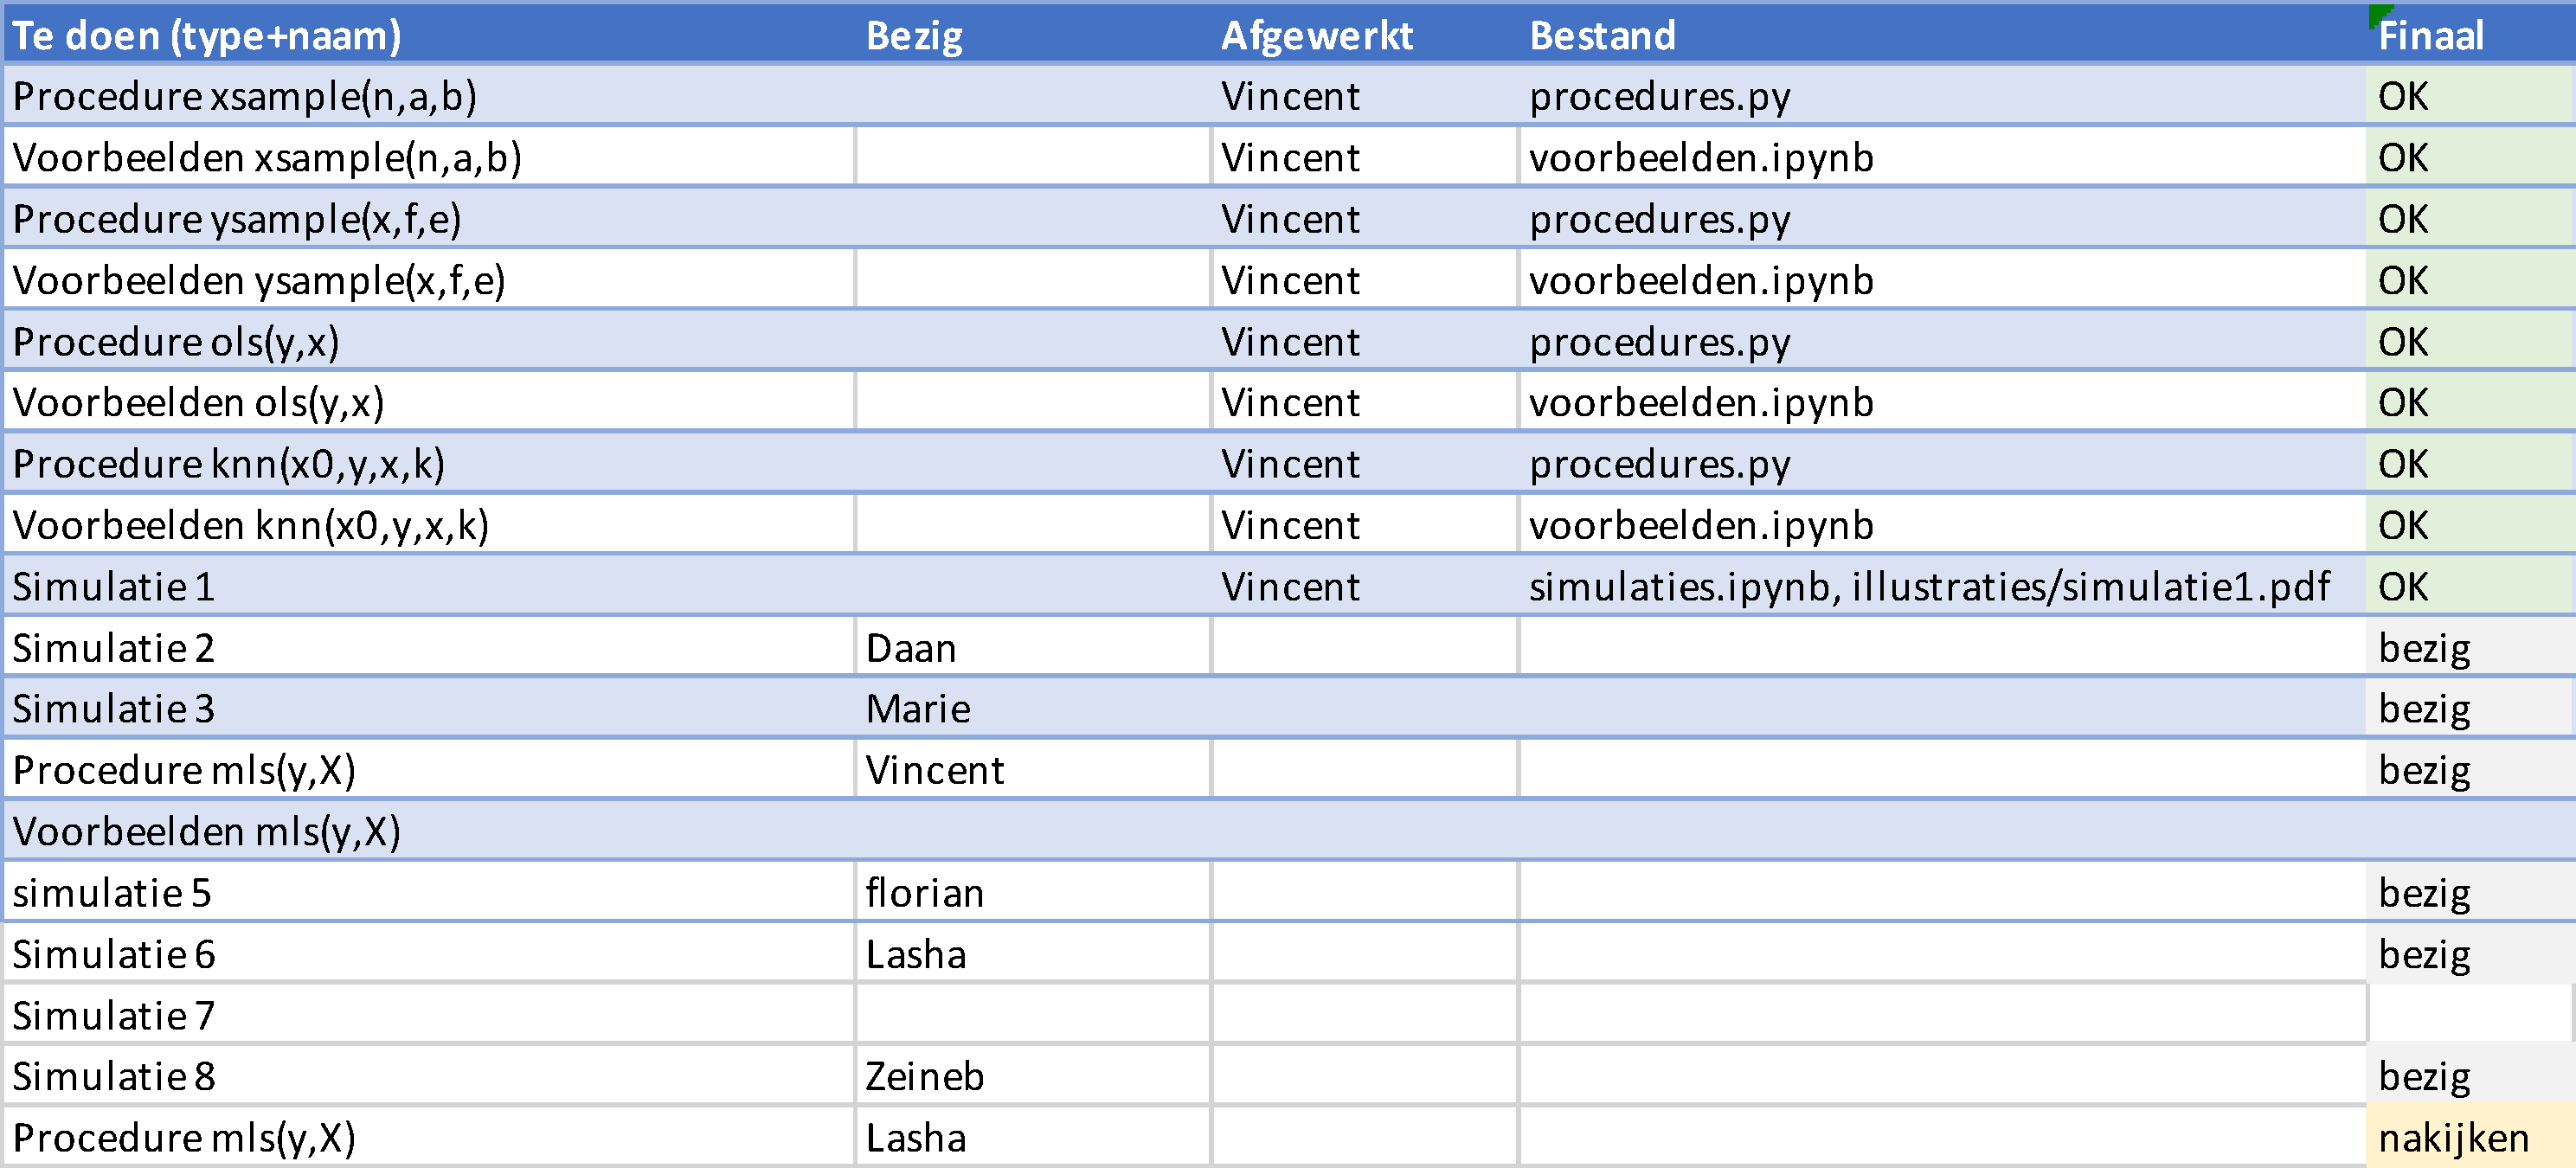
\includegraphics[width=0.8\textwidth]{kanban_einde}
	\caption{De status van het tabblad \textit{Implementatie} in de KanBan aan het einde van sessie 5}
	\label{fig:kanban}
\end{figure}

\section*{Vooruitblik}

De teamleden die startten met de implementatie van de basismethoden, zullen naar volgende week toe proberen afwerken waarmee ze bezig waren. Florian zal bovendien ook nog een oefening afwerken.

\end{document}